\chapter{Der Use Case Tresh}
\section{Entwicklung des Use Case}
Durch den ersten Teil der Arbeit, der Analyse von Rahmenbedingungen, Anforderungen und technischen Möglichkeiten für Funktechnologien von \gls{iotk} hat sich gezeigt, dass \gls{lora} in praktisch allen Bereichen eine optimales Verhältnis zu allen Anforderungen hat. Nun ist als zweiter Teil der Arbeit das Ziel, anhand eines praktischen Use Cases diese Technologie effektiv einzusetzen und dadurch erste Erfahrungen damit zu sammeln. Mit der \gls{pshmthd} soll nun ein Bedürfnis gefunden werden, welches zu der \gls{lora}-Technologie passt. Dabei kommen als erstes natürlich die Use Cases aus dem Kapitel \ref{Anwendungsfälle für IoT} zur Evaluation. Es stellte sich aber heraus, dass die meisten Use Cases den Rahmen des Projekt 2 sprengen würden. Das grösste Problem vieler Use Cases sind die verschiedenen Abhängigkeiten. So wie in den Rahmenbedingungen in Kapitel \ref{Rahmenbedingungen für iot} beschrieben, hat ein intelligentes \gls{iot}-System schnell einmal Abhängigkeiten von mehreren Sensoren und Aktoren. Die Sensoren und Aktoren haben wiederum eine Menge Schnittstellen, welche zu verbinden sind. Wir mussten feststellen, dass unser Brainstorming noch nicht zum Erfolg führte. Doch wie so oft kommen die Ideen nicht beim Brainstorming, sondern dann wenn man nicht damit rechnet: im Frust. In unserem Fall Frust über einen vollen Mülleimer. Dies brachte den Lichtblitz: Der Füllstand von Mülleimern muss überwacht werden, damit die Eimer früh genug entleert werden können und Sauereien verhindert werden können.

\begin{figure}[H]
     \centering
        \includegraphics[width=1.0\textwidth]{pictures/TRESH_Idea.png}
    \caption{Entwicklung des TRESH: vom Wägen über Lichtschranken zur Ultraschall-Distanz-Messung}
    \label{fig:TRESH Idee}
\end{figure}
Das Überwachen des Füllstandes kann ein einfacher \gls{iotk} übernehmen. Es entstehen dabei keinen Abhängigkeiten und es müssen keine Faktoren zusammengefügt werden. Ein Idealer Use Case für dieses Projekt. Als erstes musste eine sinnvolle Messmethode für den Füllstand gefunden werden. Die erste Idee: eine Waage. Dies misst jedoch das Gewicht des Mülls anstelle dessen Volumens. Lichtschranken könnten in verschiedenen Höhen des Eimers positioniert werden. Wenn die Schranken unterbrochen werden hat der Müll den Füllstand mindestens auf die Höhe dieser Schranke erreicht. Diese Messmethode scheint zuverlässig, benötigt aber ein komplexes Design des Mülleimers. Ausserdem benötigt diese Methode transparente Müllsäcke, was eher selten ist. Zudem sind die Lichtschranken in Gefahr durch den Müll verschmutzt zu werden und so bald einmal Fehlmessungen zu machen. Besser wäre es also von der Decke aus zu messen. So ist der Müllsack nicht gestört und das Risiko, dass der Sensor durch Müll verschmutzt wird ist auch viel kleiner. Für Distanz-Messungen wäre Laser eine Möglichkeit, diese misst aber nur einen Punkt, was bei den unterschiedlich grossen Müll-Elementen eher unzuverlässig ist. Ein Ultraschall-Sensor hat ein konisches Messfeld und eignet sich damit sehr gut für diese Distanz-Messung. 

\section{Markt-Recherche}
Nach der Entwicklung des Use Cases musste jetzt abgeklärt werden, ob dieser Use Case vielleicht bereits schon entdeckt und implementiert wurde. Eine Recherche im Internet nach smarten Trashes ergab, dass effektiv schon verschiedene Ideen auf dem Markt sind. Jedoch hat noch niemand ein solches Produkt entwickelt, welches die Messdaten danach auch via LoRa übermittelt. Hier ein Überblick über die gefundenen Artikel:
\begin{itemize}  
  \item GeniCan\autocite{market:genican} - der smarte Trash für die Küche scant den Barcode von Wegzuwerfenden Artikeln ein und lädt diese in eine Einkaufsliste. Eine Interessante Idee, misst jedoch nicht den Füllstand des Eimers.
  \item In London hat eine Company Namens "Renew" im Jahre 2012 sogenannte "Thank Pods"\autocite{market:LondonBins} installiert. Diese bombensicheren Mülleimer sind mit einem grossen Flachbildschirm im Hochformat ausgerüstet und sollen damit Werbefläche vermieten können. 
   \begin{figure}[H]
     \centering
        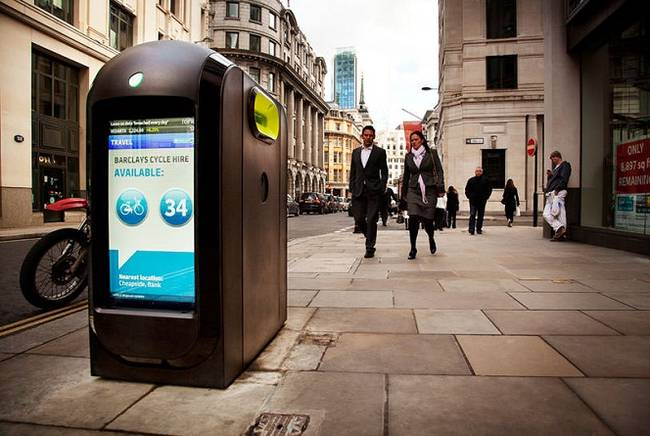
\includegraphics[scale=0.5]{pictures/London_Thank_Pod_Renew.jpg}
    \caption{"Smart bin" von "Renew" in London. Diese Smart Trashes waren Ihrer Zeit zu früh.}
    \label{fig:LondonSmartBin}
\end{figure} 
Medienberichten zufolge haben diese Pods alle vorbeigehenden WiFi-Geräte anhand der MAC-Adresse getrackt, was den Bürgern von London missfiel. Deshalb stoppte die Stadt schliesslich ein  ein Jahr später diese Mülleimer\autocite{market:LondonBinsStop}, was die Firma in den finanziellen ruin führte\autocite{market:LondonBinRuin}.
  Ob diese smarten Eimer den Füllstand auch überprüften ist in den heute noch verfügbaren Berichten leider nicht mehr nachvollziehbar. Auch die Homepage des Unternehmens (\url{renewlondon.com}) ist nicht mehr erreichbar. Offenbar war das Unternehmen damals der Zeit voraus. Heutzutage ist das Erfassen von MAC-Adressen in vieler Einkaufszentren und anderen Orten ziemlich zum Normalzustand geworden. 
  \item Auch im Jahre 2013 haben Studenten von der University of Maryland einen Smart Trash namens "Sorting Trash Can"\autocite{market:sortingTrashCan} entwickelt, welcher den Müll trennt. Sie verlassen sich dabei auf das Geräusch, welches ein Abfall beim Aufprall auf eine Platte macht. An Füllstandüberprüfung haben die Studenten jedoch nicht gedacht.
  \item In China wurden in 2015 "King Kong"-Trashes\autocite{market:ChinaTrash} installiert, welche laut Medien Feuer- und Bombensicher sind, die Müllkategorie mit Radar-Scaning erkennen und ahand davon sortieren. Weiter sind die Eimer mit einem WiFi-Hotspot ausgerüstet und angeblich versorgt ein Solarpanel diese Eimer mit Strom. Vermutlich wird der Mülleimer über 2/3/4G-Netze kommunizieren um den WiFi-Hotspot zur Verfügung zu stellen. Eine Kommunikationsleitung wäre damit schon verfügbar um einen gemessenen Füllstand zu übermitteln. Eine Medienmitteilung von einem andern Portal beschreibt auch genau dies\autocite{market:ChinaTrash2}.
  
  \item Auch in näherer Umgebung gibt es smarte Abfalleimer: In Freiburg wurden testweise 4 "Big Belly"-Mülleimer installiert\autocite{market:BigBelly}. Diese Eimer haben eine Solarbetriebene Müllpresse, welche laut eigenen Angaben das Müllkontingent des Eimers um das 7-Fache erhöht. Die Eimer können auch mit einer SIM-Karte ausgerüstet werden und so ihren Füllstand über das Mobilnetz via E-Mail mitteilen.
\end{itemize}

Bis zu dieser Recherche schien noch kein Unternehmen auf die Idee gekommen zu sein, Mülleimer "nur" mit einem Füllstandmesser auszurüsten. Stattdessen werden immer gleich "Smart-Monster" ausgeliefert, welche natürlich auch dementsprechend ein Budget kosten. Unsere Idee, einen kleinen Füllstandsensor für bestehende Mülleimer ist also immer noch auf gutem Wege. Erst als wir schon bedeutend weiter in unserer Arbeit fortgeschritten waren, entdeckten wir das Unternehmen Enevo\autocite{market:Enevo}. Diese finnishe Firma entwickelt ebenfalls einen kleinen Sensor, welcher via Ultraschall den Status eines Mülleimers misst. Was ihren Sensor jedoch teuer machen wird: die Übermittlung via das herkömliche Mobilnetz. Hier hat unsere Idee also immernoch einen Trumpf im Ärmel und gleichzeitig zeigt Enevo, dass unsere Idee definitiv eine gesuchte Lösung ist.

\section{Interview beim Tiefbauamt}
Der Use Case war nun entwickelt, der Markt recherchiert. Damit die Idee aber weiterentwickelt werden kann, ist es notwendig, Personen aus dem Umfeld zu befragen, welche Erfahrung in diesem Bereich haben. Für den Tresh eignet sich natürlich ein Tiefbauamt, welches die Müllentsorgung einer Stadt verwaltet. Wir haben aufgrund des Wohnsitzes von Simon Wittwer bei dem Tiefbauamt Thun nachgefragt. Das Tiefbauamt erklärte sich freundlicherweise einverstanden, dass wir sie interviewen durften. 
\subsection{Tiefbauamt Thun}
Das Tiefbauamt Thun hat zwei Abteilungen, welche sich mit Abfall auseinandersetzen. Das Strasseninspektorat hat einerseits die Verantwortung für saubere Strassen und in diesem Zusammenhang auch für die Leerung und Reinigung der über 500 Mülleimer und über 150 "Robidogs" in der Stadt. Im Sommer stellen sie jeweils noch einige Mülleimer zusätzlich auf, um der in dieser Saison erhöhten Müllaufkommens entgegenzuwirken. Sie haben Leerungs-touren nach Regionen und Müllaufkommen aufgeteilt. In den Ballungszentren müssen sie teilweise zweimal täglich die Eimer leeren. In den abgelegeneren Orten ist eine Leerung teilweise auch nur alle 14 Tage nötig. Teilweise müssen die Müllmänner auch vorbei, auch wenn die Eimer noch nicht voll sind. Aber als Strassenreiniger müssen sie auch das "Rundherum" des Eimers sauber halten. An den Orten mit dem höchsten Müllaufkommen haben sie 2 Mülleimer des Produktes "Big Belly" im Einsatz. Das sind dieselben Mülleimer wie in Freiburg zum Einsatz kommen. Die Übermittlung des Füllstandes interessiert sie zurzeit jedoch noch nicht, sie verwenden diese Eimer hauptsächlich aufgrund der integrierten Müllpresse um somit die Leerungs-Zyklen dank erhöhter Kapazität zu senken. Dass sie die Füllstände dieser Beiden Eimer nicht remote abrufen wollen kommt aber nicht von Desinteresse an solchen technologien, sondern macht bei 2 Eimern einerseits noch keinen Sinn und andererseits befinden sich die Eimer sowieso an den Orten, wo die Leerungen täglich stattfinden.

Die Technischen Betriebe haben andererseits einen Disponent Abfallentsorgung. Dieser organisiert und verwaltet die Container- und Unterflur-Anlagen, welche die Stadt für die Hauskehricht- und Papier-Entsorgung betreibt. Glas und Aluminium wird interessanterweise nicht von der Stadt, sondern von einer Privatfirma, der AVAG übernommen.
Auch bei diesen Containern hat das Tiefbauamt bereits Erfahrungen mit ersten \gls{iot}-Versuchen gemacht. vor 4 Jahren hatte eine Firma Ultraschall-Sensoren zur Messung der Füllstände installiert. Leider ohne Erfolg, die Sensoren lieferten falsche Messresultate und meldeten, dass der Container voll sei, auch wenn er erst halbvoll war. Das vermutlich aufgrund von "Bergbildung" innerhalb des Containers. Das heisst, der herabfallende Müll bildete eine Pyramide, dessen Spitze vom Sensor erfasst wurde und deshalb den Container als voll meldete. Aufgrund dieses Misserfolges war das Amt natürlich enttäuscht, über die Technologie und "etwas gebrannt" davon. Sie verstehen aber auch, dass in 4 Jahren "die Technologie wieder Fortschritte gemacht hat" und sind deshalb nicht abgeneigt für neue Sensoren.

\subsection{Resultate aus dem Interview}
Das Konstruktive Interview mit den Herren des Tiefbauamts brachte uns viele Inputs welche wir für den weiteren Verlauf des Projektes mitnehmen.
Da es beidseitig nicht ganz einfach war einen Termin zu finden, mussten wir allerdings bereits mit der Entwicklung des Prototyps beginnen, bevor wir das Interview durchführen konnten. Deshalb konnten Informationen und das Feedback von den Herren leider nicht mehr in den Prototypen einfliessen. Wir nehmen dieses Wissen aber mit für einen eventuellen Nachfolgeprototypen in der Bachelorarbeit. Folgende Punkte halten wir fest:
\begin{itemize}  
  \item Für ein Strasseninspektorat spielt nicht nur der Füllstand eines Mülleimers eine Rolle. Auch die Umgebung um den Mülleimer muss sauber sein. Optimal wäre dazu natürlich eine Kamera, welche die Umgebung periodisch fotografiert. Energietechnisch und für das Übertragen der Daten ist eine Kamera jedoch suboptimal und weiter käme die Frage, wo die Kamera aufgestellt werden kann. Statt einer Kamera könnte jedoch ein Feedback-System beim Eimer eingebaut werden. Vorbeigehende Passanten treffen eine Frage auf dem Eimer an: "Ist's hier sauber?" und können mit einem "Daumen hoch"- oder "Daumen runter"-Knopf darauf antworten. Dadurch könnten Quasi die Passanten die Augen für das Reinigungsteam spielen.
  \item Für die Müllmänner wäre trotz der Remote-Füllstand-Überwachung auch eine lokale Füllstand-Anzeige sehr praktisch. Wenn sie gerade vor Ort sind müssten sie nicht den Müll öffnen um dessen Füllstand zu überprüfen, sondern könnten nur die Anzeige (beispielsweise eine LED) kontrollieren. Wenn dann jeder Müllman ein Smartphone mit einer Leerungs-App hat entfällt dieser PUnkt natürlich wieder.
  \item Die Sensoren müssen Vandalen- und Witterungs-Sicher sein. Da die Mülleimer jeweils mit Hochdurckreinigern geputzt werden, braucht es eine gute Wasserdichtheit.
  \item Für Container reicht nicht nur ein Einzelner Ultraschall-Sensor. Entweder mehrere verteilte Ultraschall-Sensoren, oder aber andere Messemthoden sind hier gefragt.
\end{itemize}
